%=======================================================================
% Unix One: An Introduction to the Unix Command Interface
% for the Linux Initiative
% Faculty of Engineering, University of Peradeniya
% Visvanath Ratnaweera
% Created: January 2015
% Version: Jan/Feb 2017
%=======================================================================
\documentclass[11pt,a4paper,twoside]{article}

%===== packages =====
\usepackage[dvips]{graphicx}
\usepackage{pst-all}
\usepackage{pst-circ}
\usepackage{listings}
\usepackage{hyperref}
\usepackage{fancyhdr}
\usepackage{datetime}

% ===== Paper layout control =====
\setlength  {\voffset}          {0mm}
\setlength  {\hoffset}          {0mm}
\setlength  {\topmargin}        {0mm}
\setlength  {\headheight}       {12pt}
\setlength  {\headsep}          {2mm}
\setlength  {\textwidth}        {155mm}
\setlength  {\textheight}       {230mm}
\setlength  {\marginparwidth}   {30mm}
\setlength  {\marginparsep}     {3mm}
\setlength  {\oddsidemargin}    {5mm}
\setlength  {\evensidemargin}   {-5mm}
\setlength  {\parskip}          {2mm}
\setlength  {\parindent}        {0mm}

%=== document info ===
\begin{document}

\title{Unix One: An Introduction to the \\ Unix Command Interface}

\author{\\ Visvanath Ratnaweera \\
\\
For the Linux Initiative \\ Faculty of Engineering, University of Peradeniya \\
\\ }
\date{11 January - 14 February 2017 \\
Course URL: \url{https://feels.pdn.ac.lk/course/view.php?id=346}}

\maketitle
\thispagestyle{empty}

\begin{abstract}
'Unix One' will take someone with no knowledge of Unix commands to being 
able to move confidently in a text terminal. 

Through completion of class work the participants will be able to:
\begin{itemize}

\item get information about the Unix system environment

\item refer the built-in help mechanisms

\item navigate directories in a file system

\item do simple file manipulations

\item edit and manupulate text

\item communicate with other shell users in the same system

\end{itemize}
\end{abstract}

\newpage

\setcounter{page}{1}
\pagestyle{fancy}
\fancyhead{}
\fancyfoot{}
\renewcommand{\headrulewidth}{0pt}
\renewcommand{\dateseparator}{-}
\fancyfoot[LO,RE]{Unix One (\yyyymmdddate\today\ \currenttime)}
\fancyfoot[LE,RO]{\thepage}

\setcounter{tocdepth}{2}
\tableofcontents
\pagenumbering{roman}

\newpage

%============================ Intro ================================
\section{Introduction, Your first log in}
\setcounter{page}{1}
\pagenumbering{arabic}

You will get a shell account, which you can access from anywhere in the
faculty network, or in two steps from anywhere in the Internet. To access
the shell you need a terminal emulator on your machine. In the process you 
familiarize yourself with terms like terminal, remote log in, shell, 
prompt, etc.

\subsection{Why use a command interface}

\begin{figure}[htb]
  \begin{center}
    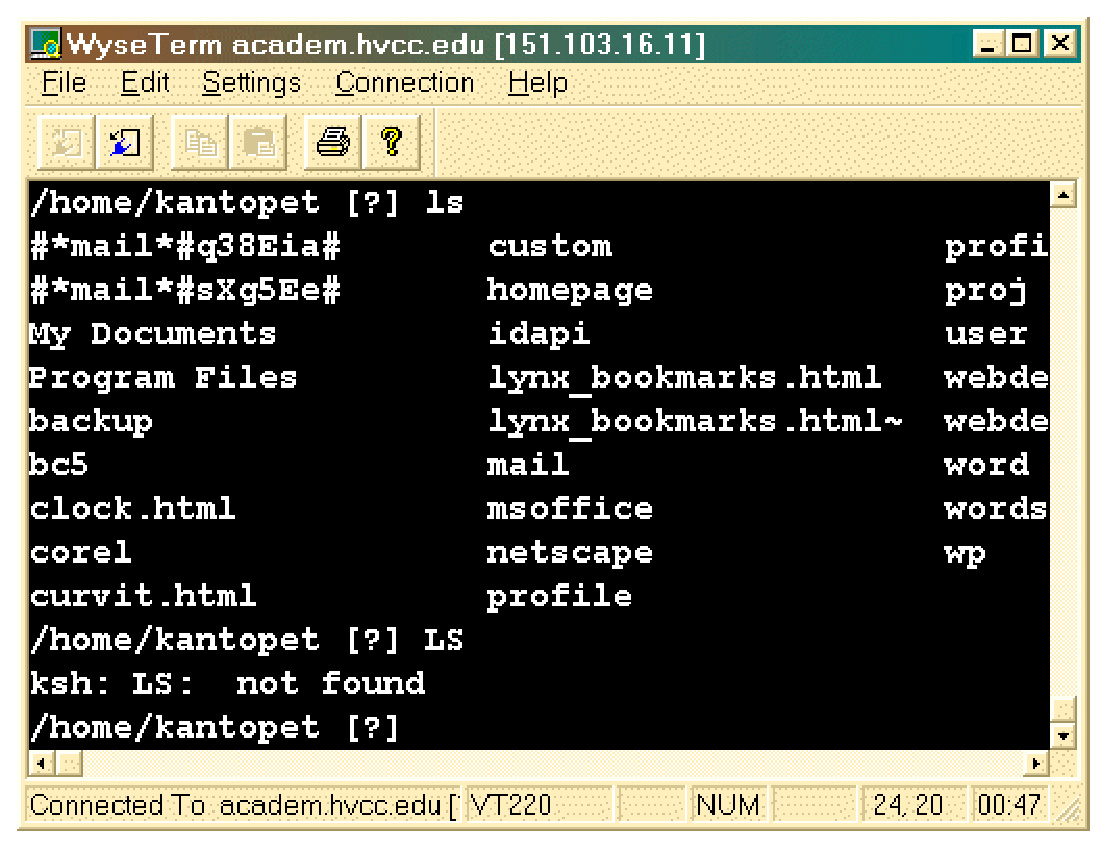
\includegraphics[width=10cm]{images/scr_casesense}
    \caption{A terminal session}
  \end{center}
\end{figure}

Experienced system administrators maintain their machines from the command 
prompt. They compile source code, install programs, troubleshoot their 
operation, automate routine tasks; all in this text environment. Unix relies 
heavily on text, whether in the form of configuration files or as scripts, 
and Unix masters an elaborate system of pattern matching in text called 
\emph{regular expressions}. The Unix command language is also a programming 
language. One can write interactive programs in this language or paste other
specialized programs together in scripts or pack routine tasks into scripts 
and schedule them to run regularly.

Graphical User Interfaces (GUI) are convenient but they don't tell you 
exactly what they do behind the interface. Once something unexpected 
happens or if you have a task for which there is no option in the GUI, 
you are stuck. In addition to that the text terminal doesn't require the 
overhead a GUI needs which is a critical factor in remote administration. 


\subsection{Your login to the Unix shell}
%----------------------------------------

In the early days people went to great lengths to access a Unix terminal. 
Only the system administrators had access to the system console itself.
Users accessed the machine through terminals - in the same building 
through serial lines or from a distances through telephone 
lines\footnote{See unit 1 of the preliminary course History of FOSS}. 
The machines were simply too expensive to be duplicated!

Today it is the opposite. Computers are everywhere! Because of their
diversity there are also numerous ways of accessing them. There lies a 
problem for the beginner. Even within Unix the multitude of flavours 
make them seemingly different to each other. Which means that the 
inexperienced can not rely on the exact behaviour of individual examples.

\begin{figure}[htb]
  \begin{center}
    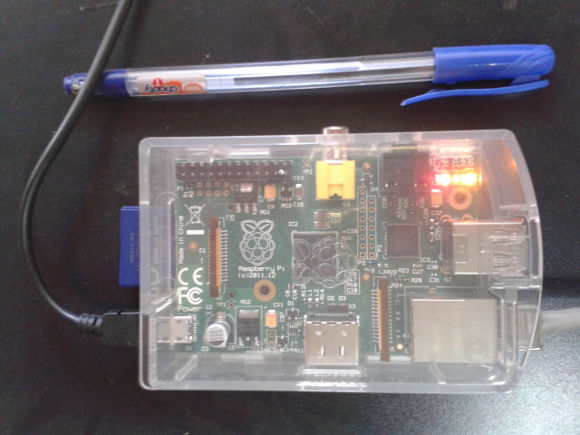
\includegraphics[width=8cm]{images/20150126_152213_scaled}
    \caption{The Raspberry Pi miniature computer}
  \end{center}
\end{figure}

Therefore in this course all the participants will be working together in 
the same enviroment - in a Raspberry Pi running a Debian GNU/Linux port, 
which you access remotely through the network. (See the assignment of this 
week for details.)

\subsection{Your first login}
%----------------------------

Typically a Unix terminal ``greets'' the user by printing something about 
itself on the screen and then requests the user to identify himself:

\begin{figure}[htb]
  \begin{center}
    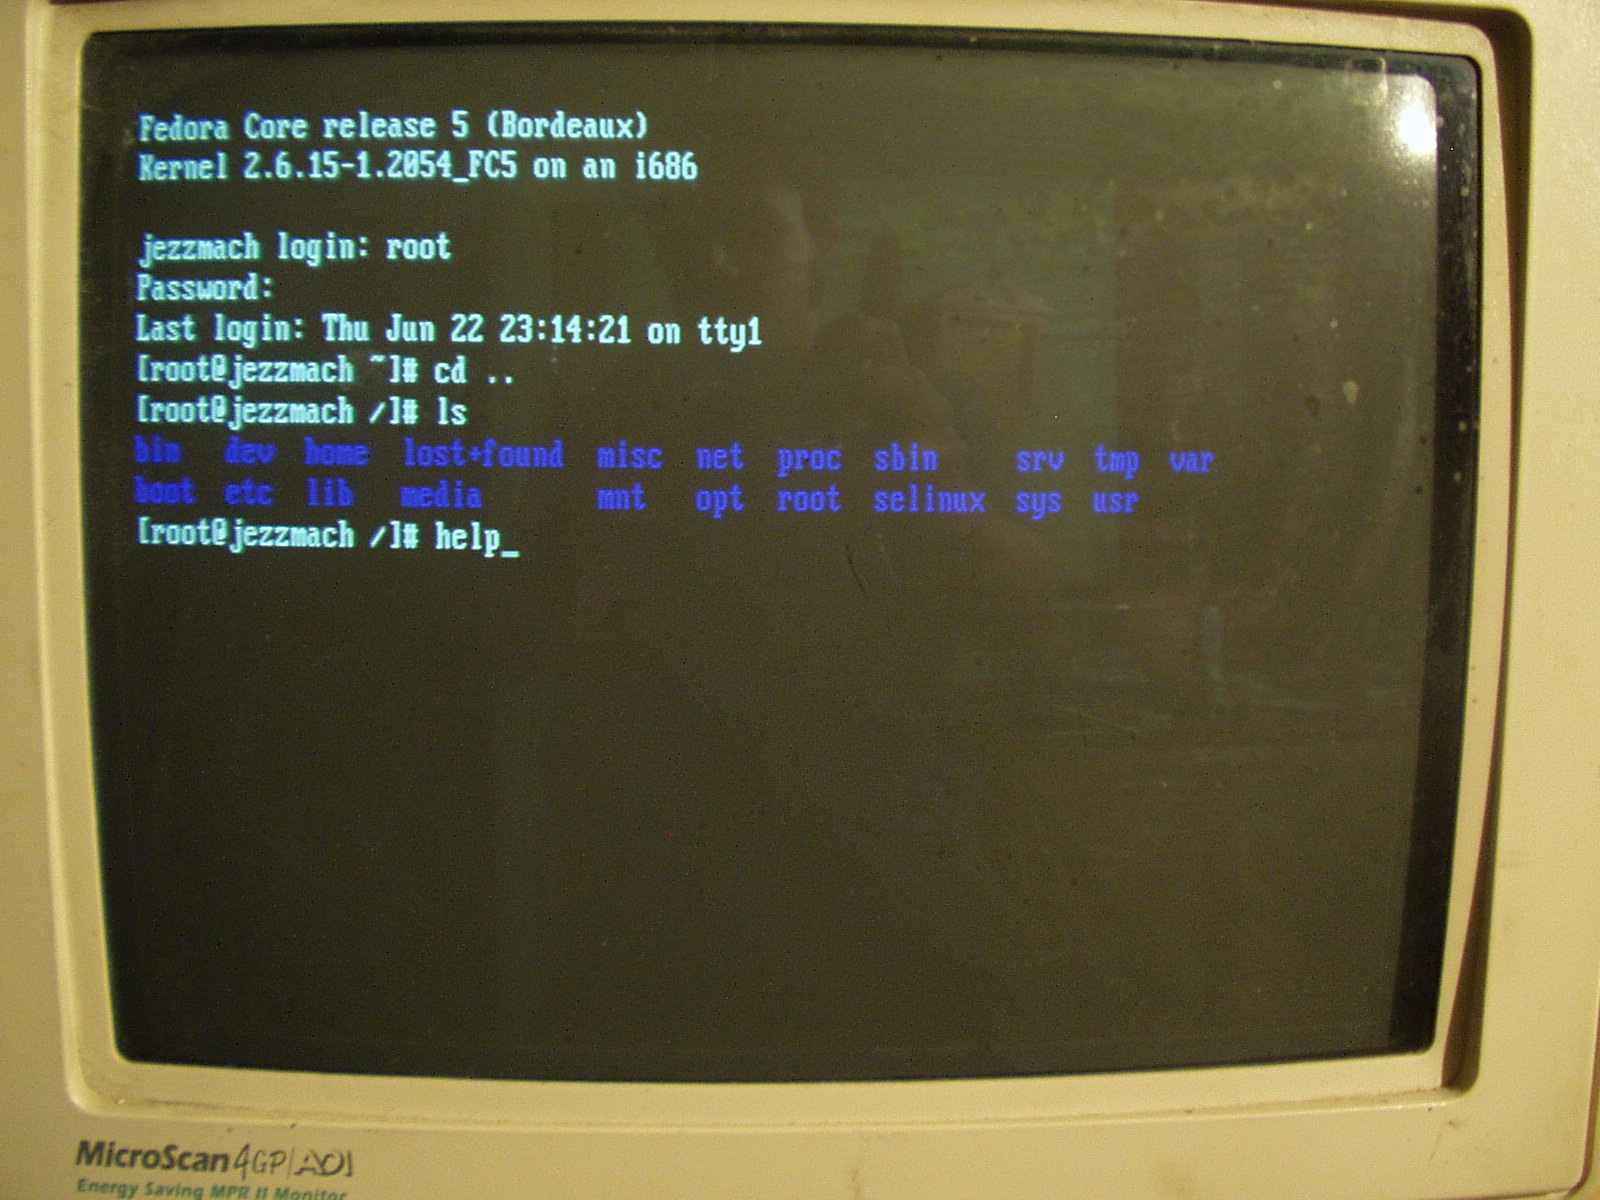
\includegraphics[width=10cm]{images/fedora_console}
    \caption{A terminal session}
  \end{center}
\end{figure}

The terminal shown in the above figure has printed the Unix flavour, the 
version number of the kernel, the machine architecture and the host name. 
Then it requests the user to identify himself by presenting him with a 
\emph{login prompt}. The user has to sign in by entering his login name 
and the password. Here is another example:

\begin{lstlisting}[frame=single]
CrunchBang Linux waldorf cherry tty4
Kernel 3.13 on an i686
cherry login: john
Password: [suppressed]
Last login: Mon Feb 29 12:34:56 on tty6
Linux cherry 3.2.0-4-amd64 
[...]
john@cherry:~$
\end{lstlisting}

The first lesson: Unix is case sensitive! Don't type \texttt{John}, if 
your login name is \texttt{john}. This might come as a surprise for the 
typical MS Windows user, but Unix was case sensitive right from the beginning 
with a strong orientation towards lower case - supposedly for easy typing.

The original terminals used serial connections, as a result there were
many switches to be set - transmission speed or \emph{baud rate}, handshake
method, duplex method (full or half), etc. - and even required handling a 
telephone! That was magic which didn't work without the help of a local 
expert. The result of all that effort was to get the login prompt.

Today the world is different. Most of the users have a Microsoft Windows 
desktop in front of them and they want to connect to the Unix across the
Internet.  If you are one of them get the free terminal emulator program 
PuTTY from its site 
\footnote{\url{http://www.chiark.greenend.org.uk/~sgtatham/putty/}}. 
Just copy the 'exe' file to any directory and run it! You might want to 
make a profile (Figure 2) so that you don't have to enter the same 
information every time.
\begin{figure}[htb]
  \begin{center}
    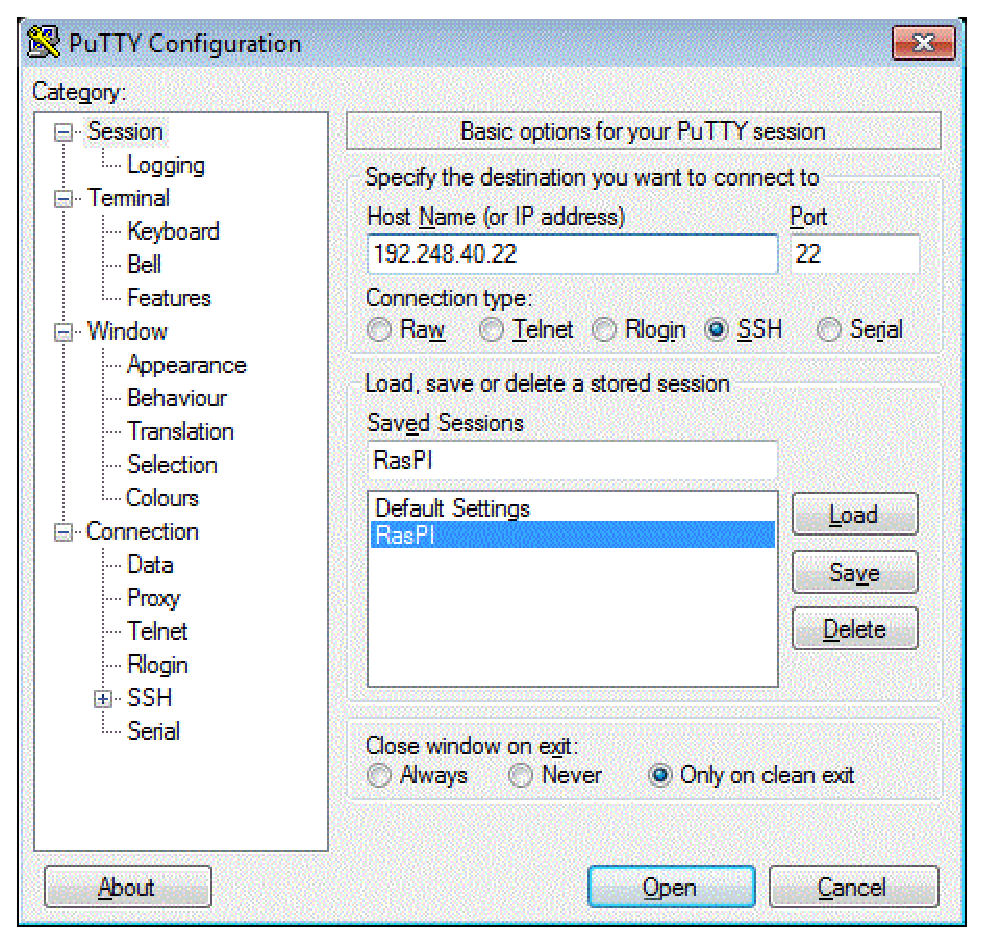
\includegraphics[width=10cm]{images/putty}
    \caption{Setting up PuTTY}
  \end{center}
\end{figure}

If you are on a Unix machine like Mac or Linux, you definitely have a 
terminal \textsl{emulator}. Look for a program called Terminal, Konsole,
Command, or something similar. What you need is just the SSH client, 
which is unimpressively called \texttt{ssh}. Try 
\texttt{ssh \emph{login}@\emph{host}} at the command prompt.  (Here 
\texttt{\emph{login}} stand for you login name; the \texttt{\emph{host}} 
is the DNS name or the IP address of the host. 

\begin{figure}[htb]
  \begin{center}
    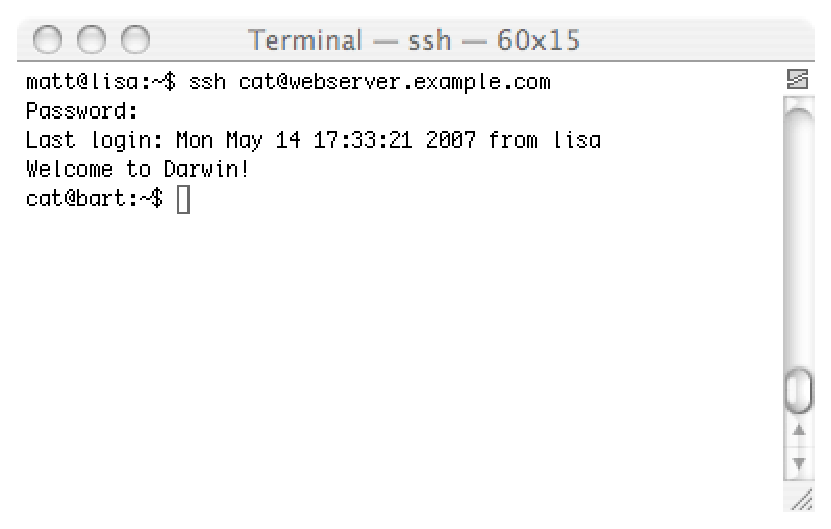
\includegraphics[width=10cm]{images/macos-logged-in}
    \caption{Connecting from Mac OS X or Linux}
  \end{center}
\end{figure}

In all these cases, the first time you log in you will get a warning about
establishing the authenticity of the host. Accept it only if the finger
print is correct, in the case of our 'arm' it is 
22:2f:cd:f3:df:d1:af:5d:66:dc:c0:74:68:86:14:22.

Once successfully logged in, the login procedure starts an interpreter 
which will be ``talking'' to you. This is called the \emph{shell}. 
The shell signals that it is listening by printing its \emph{prompt}. 
In the example above \texttt{john@cherry:\~\$} is the shell prompt. Certain 
information in it are easily guessed. Note the general format 
\texttt{login@host}, which we are going to encounter often.

Also note that the default shell prompt vary from system to system. Since 
the user can customize it anyway, in this documentation we use simply the 
'\texttt{\$}' character as the shell prompt.

You can now start working in Unix.

\subsection{Changing the password}
You should change the initial password you received from the system 
administrator to one of your own. You enter the command \texttt{passwd} 
to change your password:

\begin{lstlisting}[frame=single]
$ passwd
Changing password for john.
(current) UNIX password: 
Enter new UNIX password:
Retype new UNIX password:
passwd: password changed
\end{lstlisting}

When changing password not only that you should know the old password but 
you need to type the new password twice. Also notice that certain systems 
may have restrictions on the password like minimum length and whether you 
must use digits and/or special characters.

Note that the superuser can change password without providing the current
password.  Which means that the superuser can not find out the current 
password of a user, he can only set it to a new value.


\subsection{Logging out}
%-----------------------
The command to log out is, you guessed it, \texttt{logout}. It instructs 
the shell to terminate your session. That will close the shell and reset 
the terminal so that it will fall back to the login prompt you saw at the 
beginning. Try it!

On a side note: It is not meaningfull to shut down the machine as a 
normal user: this is obviously something for the superuser!

\subsection{Assignment 1}

Step 1: If you are on Windows, install a terminal emulator like PuTTY and 
then log in to either aiken.ce.pdn.ac.lk or tesla.ce.pdn.ac.lk. If you are 
on a Unix you can simply type 'ssh eNUMBER@server.name' in a terminal.

From there login to the 'arm', a Raspberry Pi, by entering 
'ssh eNUMBER@arm.ce.pdn.ac.lk'.

Step 2: Take a screen-shot just after logging in and upload it to the 
assignment tool.

\subsection*{Summary}
In this week you have learned:
\begin{itemize}
\item the advantages of the Unix command interface

\item the difference between the console and a terminal

\item the more common remote login over the network

\item to recognize the login prompt of a Unix terminal

\item to recognize a Unix shell prompt

\item to remotely log in to a Unix shell through the network

\end{itemize}

\newpage

%=============================== Section 2 =============================
\section{A session with Unix}
%----------------------------

In this unid you will go through a longer session with Unix to get to 
know the system and the terminal a bit better.

From the time you logged on to the system you are "on session" until you
log out. As you read this section try those commands yourself in the newly 
recieved shell account!

\subsection{Exploring your system environment}

\subsubsection{Viewing the system date and time}

Users can display the system's current date and time using the \texttt{date} 
command:
\begin{lstlisting}[frame=single]
$ date
Thu Feb 29 21:21:12 IST 2015
\end{lstlisting}

The date string above might look strange to you. It is the format originally
chosen by the inventors of Unix and still the default format in most of the
Unix-like systems. To change the format give the \texttt{date} command a 
format string as an option. Here are some examples:

\begin{lstlisting}[frame=single]
$ date "+%T"
21:21:12
$ date "+%Y"
2015
\end{lstlisting}

Make a note of the timezone in the earlier example. In that IST stands for 
Indian Standard Time, which is also the time observed in Sri Lanka. IST is 
5 h 30 min ahead of UTC, Coordinated Universal Time. Typically a Unix system's
hardware clock is synchronized to UTC. The system knows the local time from 
its timezone setting. (And if you carry a computer across timezones, you 
switch the timezone, not the system clock!)

The original designers of Unix have arbirtraliy chosen the instant
00:00:00 UTC of 1 January 1970 as the origin of its system time or the 
``epoch''. This has become a part of the Unix standard and is widely 
used. You can get the this \emph{epoch time} in seconds by running 
\texttt{date "+\%s"}.

The \texttt{date} command can also change the system time, but only the
system administrator is allowed do that. In fact, Unix systems rely much
on accurate clock time and therefore almost always synchronized with a 
time server. But system administration is out of scope right now.


\subsubsection{Monthly calenders}

The standard calender program of Unix is called \texttt{cal}:

\begin{lstlisting}[frame=single]
$ cal
    January 2015      
Su Mo Tu We Th Fr Sa  
             1  2  3  
 4  5  6  7  8  9 10  
11 12 13 14 15 16 17  
18 19 20 21 22 23 24  
25 26 27 28 29 30 31  
                      
\end{lstlisting}

The program \texttt{ncal} offers you an alternative layout. Try 
\texttt{cal -3} and \texttt{ncal -3}.

\subsubsection{How busy is the machine}

There is another time-related command called \texttt{uptime} which shows the
duration for which the system has been running. In addition it tells you how
many users are currently logged in and prints out three values for system load 
averages: the load average during the last 1, 5 and 15 minutes.

\begin{lstlisting}[frame=single]
$ uptime
 17:19:20 up 13:34, 6 users, load average: 0.22, 0.18, 0.15
\end{lstlisting}

The unit of measurement for load average is the number of CPUs (or 
hyperthreads) being utilized. If the machine is single CPU 1.00 means 
the CPU is fully utilized, if it has 2 CPUs, each with two hyperthreds a 
value of 4.00 means that all four CPU threads are being fully utilized. 
(Well, there is more to it. For now we have to leave it at that.)

There is another famous command called \texttt{top} which continously 
monitors the system state:

\begin{lstlisting}[frame=single]
top - 17:52:46 up  1:42,  7 users,  load average: 0.10, 0.09, 0.12
Tasks: 157 total,  2 running, 155 sleeping, 0 stopped,   0 zombie
Cpu(s):  1.0 us,  1.1 sy,  0.0 ni, 97.8 id,  0.1 wa,  0.0 hi,  ...
KiB Mem:  7987388 total, 1825888 used, 6161500 free,  79584 buffers
KiB Swap:       0 total,       0 used,       0 free, 854744 cached

  PID USER   PR  NI  VIRT  RES  SHR S  %CPU %MEM    TIME+  COMMAND           
 2950 root   20   0  162m  22m 6884 S   5.0  0.3   2:49.21 Xorg              
 7829 foo    20   0  416m  34m  16m S   1.0  0.4   0:00.29 termin   
 6863 bar    20   0  468m  49m  14m S   0.7  0.6   1:06.15 evince            
 [...]
\end{lstlisting}


\subsubsection{System information}

The system's DNS name can be querried through the command \texttt{hostname}. 
The command \texttt{uname} prints system information like the CPU architecture 
and the operating system:

\begin{lstlisting}[frame=single]
$ hostname
arm
$ uname -a
Linux arm 4.4.11+ #709 SMP Mon May 23 15:28:00 BST 2016 \ 
  armv6l GNU/Linux
\end{lstlisting}

Another source of system information are called \emph{environment variables}.
This is an area in the memory space of the shell where a list of variables
and their values are stored. One can querry them with the \texttt{echo} 
command. The value of a variable is addressed by prepending its name by 
the \$-sign:

\begin{lstlisting}[frame=single]
$ echo $OSTYPE
linux-gnu
$ echo $SHELL
/bin/bash
\end{lstlisting}

Some other useful environment variables are: HOSTNAME, HOSTTYPE, TERM, 
USER. Try them! 

Note that traditionally the environment variables are written in all capital. 



\subsection{Screen handling}

\subsubsection{Type-ahead}

The terminal emulator reads the keys you type as you type them immediately
pass them to the (remote) shell. The keys are normally ``echoed'' back to 
the terminal unless they are suppressed as in the case of passwords. If the 
shell is busy with something else or the connection is very slow, you might 
not see the echo immediately. But you don't need to worry. The keys strokes
are put to a queue and the shell answers wenn it is back. Which means, you 
can type blindly ahead of the shell output.

You can think of the keys strokes and the output of the shell as two 
independent streams of characters. They do not get in to the way of
the other!

\subsubsection{Modifying the screen}

If too much text is printed on terminal the \texttt{clear} command 
will clear it. Also watch the behaviour of the simple Enter key. In
fact, it is a simple way of testing whether a shell is responding.

Programs may send special characters to the terminal to get various
effects like colour or blinking text. Sometimes this leads to mishaps, 
where the display gets completely messed up. With the \texttt{reset} 
command you can recover, but you may have to type it blindly!

The original terminals had fixed sized fonts. Which meant that for a
given resolution of the terminal the number of characters per line 
(called columns) and the number of lines displayed were always the 
same: 80 columns times  24 lines was a common standard. In today's 
high resolution graphics there is no such correlation. 

You can querry the terminal size through the \texttt{resize} command.

\begin{lstlisting}[frame=single]
$ resize
COLUMNS=92;
LINES=27;
export COLUMNS LINES;
\end{lstlisting}


\subsubsection{Control keys}

In dedicated terminals there was a BREAK key to stop whatever the command
is running at that moment. Later this funtion was taken over by the
Delete key. In todays keyboards the Delete key deletes the last character 
you typed. As you can see these things are system dependent. But a set
of commands known as Control commands have a faily consistant behaviour
throughout many systems.

You can break a running program by typing \texttt{Ctrl+c}. To delete a
character, the equivalent to Delete, \texttt{ctrl+h}. \texttt{ctrl+u}
deletes whole command line to the left of the cursor, \texttt{ctrl+k}
kills the part to the right of it. \texttt{ctrl+d} signals the end of
input, which will close the shell. Or, if you just want the output to 
pause, to keep something important disappearing off the screen, type 
\texttt{Ctrl+s}, the pause. To restart type \texttt{Ctrl+q}.

The following table lists some of the more important Ctrl keys.
\begin{center}
\begin{tabular}{ l | l }
\hline
Shortcut & Effect \\
\hline
Ctrl-a & Go to the beginning of the line \\
Ctrl-c & Kill the current process \\
Ctrl-d & (on a line of its own) Exit the current shell \\
 & (otherwise) delete the character under the cursor \\
Ctrl-e & Go to the end of the line \\
Ctrl-h & Delete the character to the left of the cursor (backspace) \\
Ctrl-k & Delete from the cursor position to the end of line \\
Ctrl-l & Clear the screen \\
Ctrl-u & Delete from beginning of line to cursor position \\
%Ctrl-w & Deletes the word before the cursor \\
%Ctrl-z & Suspend the current process and put it to background \\
\hline
\end{tabular}
\end{center}

\subsection{More about ending the session}

In the previous unit we said that the command \texttt{logout} is the
right way to log out. Strictly speaking this is not right. You can
log out only from the very first shell the login process gave you.
You could have started more shells on top of it. (You just start
another shell by typing its name. Try \texttt{bash} or \texttt{dash},
names of available shells.) Before you log out, you need to cloase
those shells. The proper way to do that is to type \texttt{ctrl+d}
(or \texttt{exit}). The ``exit'' from the last shell will automatically
logs you out!


\subsection{Assignment 2}

Preparation: When capturing a screen-cast the typical GUI user makes HD 
films, generating huge files which are sometimes not even sharp. The 
shell user captures his terminal in the terminal itself. The resulting 
files are thousand times smaller and always sharp!

This is quite easy: There are many terminal recording tools. We will use 
\texttt{ttyrec}. Just by issuing the command \texttt{ttyrec} it will begin 
capturing everything that happens in the terminal to a file. To end the 
capture, type \texttt{exit}. You will find the recording in a file called 
\texttt{ttyrecord}. To give it a different name, simply provide the file 
name as a parameter.  For example:

\begin{lstlisting}[frame=single]
$ ttyrec  mywork.ttyrec
[work in the terminal]
$ exit
exit
\end{lstlisting}

Please be careful not to press non-printable keys like arrows during the
recording. They tend to upset the recording!

To play back, run:
\begin{lstlisting}[frame=single]
$ ttyplay mywork.ttyrec
\end{lstlisting}

Assignment: Login to your shell account and first go through the steps 
given below. Once you are confident capture your work to a file named 
eNNNNN\_assignment2.ttyrec. If you still make a mistake, just start ttyrec 
again with the same file name.

Step 1. Display the system clock time.

Step 2. How many seconds have passed from 00:00:00 UTC of 1 January 1970 to the
time you are doing the assignment?

Step 3. Display the output of uptime.

Step 4. Get the values of the environment variables HOSTNAME, HOSTTYPE, USER
and HOME?

Step 5. Clear the screen.

Step 6. Find the size of your terminal in columns x lines. Hint: resize.

Now exit the ttyrec. Check the recording by running ttyplay. If everything is
OK then go back to the Assignment in Moodle, write a note saying that
you have finished the assignment. (You don't have to upload anything, the
superuser can play back the script file.)

\subsection*{Summary}
%------------------------------
\begin{itemize}
\item You know that the system clocks of Unix computers are synchronized
to UTC and they calculate the local time from their timezones.

\item That the time keeper of Unix ticks relative to the ``epoch'', which was
00:00:00 UTC on 1 January 1970.

\item Simple usage of the commands \texttt{date}, \texttt{cal} and 
\texttt{ncal}.

\item Can get information about the operating system and the working 
environment from the commands \texttt{hostname}, \texttt{uname} and the 
environment variables OSTYPE, HOSTNAME, HOSTTYPE, SHELL, TERM.

\item You know that the terminals measure their resolution in no. of columns
x no. of lines - 80x24 being the standard - and that you can querry your 
terminal program with the \texttt{resize} command.


\end{itemize}

\newpage

%============================== Section 2 =============================
\section{Getting help from the system itself}

In this chapter you'll be introduced to:
\begin{itemize}
\item the \emph{manual pages} and the \emph{GNU Info}, the two primary 
documentation systems which should be built into any Unix system

\item the \texttt{--help} option provided by almost all the command line 
tools and the \texttt{help} command of the shell

\item \emph{command completion} and \emph{command history} - two features 
which greatly simplify your typing. 

\end{itemize}

\subsection{The manual pages}
%------------------------------
The original \emph{UNIX Programmer's Manual} documents the sytem divided 
into nine sections: Section 1 deals with the commands for the end user,
the commands we discuss in this course. Incidentally games too were a 
part of the system, section 6 contains information on games.  The remaining
sections handle details which are aimed for the programmer and the system 
administrator.  This documentation was always a part of the system.

The \texttt{man} program searches, formats, and displays the information
contained in those manual pages. Because many topics have a lot of information, 
output is piped through a terminal pager program for convenient viewing
one page at a time; at the same time the information is formatted for a good 
visual display. You can call \texttt{man} just by giving the name of the 
program which would like to know more about. For example:

\begin{lstlisting}[frame=single]
$ man uname
UNAME(1)                         User Commands                        UNAME(1)

NAME
  uname - print system information

SYNOPSIS
  uname [OPTION]...

DESCRIPTION
  Print certain system information.  With no OPTION, same as -s.

  -a, --all
    print all information, in the following order, except omit -p
    and -i if unknown:

  -s, --kernel-name
    print the kernel name
[...]
\end{lstlisting}

The output says that the page is from section 1 'User Commands' and
explains its usage. 

Note that the man pages have a well defined structure, part of which is 
listed in next table. Thanks to their structure the man pages can be 
automatically converted to HTML, to book form or to graphical help programs.
You will encounter them if you continue working in the shell after the 
course, but during this course we expect you to refer the local man pages 
with the help of \texttt{man}.

\begin{center}
\begin{tabular}{ l | l }
\hline
Item & Description \\
\hline
SYNOPSIS & Command usage along with the optional and non-optional arguments \\
DESCRIPTION & Details on how to use the command and and explanation of each
section \\
EXAMPLE & Examples of how to use the command \\
FILES & Files that have to be available for this command to work \\
SEE ALSO & Commands that are similar in purpose \\
DIAGNOSTICS & Explanation of error messages \\
WARNINGS & Things to be careful about when using the command \\
BUGS & Known problems and suggested improvements \\
\hline
\end{tabular}
\end{center}

For reading long manual pages on screen \texttt{man} delivers them
through a pager, which depends on the Unix flavour. The pager used in
Linux is called \texttt{less}. You navigate in \texttt{less} with single 
key strokes: f, Ctrl+f or space bar to scroll page-wise forward or b, 
Ctrl+b, or Shift+space to scroll back and 'q' for quit. The key 'h' gives 
your the the full list of commands.

Another useful key is \texttt{/} (forward slash), the search key. Often
all you need to know is what a specific option of a command does, for
example what 'uname -s' really means. In such cases just call 'man uname'
and then press \texttt{/ - s}. If the first hit is not the one you were looking
for, keep on pressing \texttt{n} (for next).

Exercise. Call the man pages of the commands you already know and note
down options you find interesting. Don't forget 'man man' too!

By default the \texttt{man} command prints only the dedicated page
specifically about the topic. You can broaden this to view all man pages
containing a particular string in their name by using the -f option. 
The following dialog shows that there is only one \texttt{date} command
whereas there are two \texttt{time} commands.

\begin{lstlisting}[frame=single]
$ man -f date
date (1)     - print or set the system date and time
$ man -f time
time (7)     - overview of time and timers
time (2)     - get time in seconds
\end{lstlisting}

You select the section of the manual by giving its number as an optin:

\begin{lstlisting}[frame=single]
$ man 2 time
TIME(2)               Linux Programmer's Manual              TIME(2)

NAME
  time - get time in seconds
[...]

$ man 7 time
TIME(7)               Linux Programmer's Manual              TIME(7)

NAME
  time - overview of time and timers
[...]
\end{lstlisting}

You get the same effect of 'man -f' by the command \texttt{whatis}.

\begin{lstlisting}[frame=single]
$ whatis time
time (7)     - overview of time and timers
time (2)     - get time in seconds
\end{lstlisting}

A common problem with the man command is that you need to know the
name of the command you want to know more about. The -k option broaden
the search by including all commands whose description contains the
search string:

\begin{lstlisting}[frame=single]
$ man -f  user
user: nothing appropriate.
$ man -k user
adduser.conf (5) - configuration file for adduser(8) and addgroup(8)
deluser.conf (5) - configuration file for deluser(8) and delgroup(8)
[...]
\end{lstlisting}

The \texttt{apropos} command is equivalent to 'man -k':
\begin{lstlisting}[frame=single]
$ apropos user
adduser.conf (5) - configuration file for adduser(8) and addgroup(8)
deluser.conf (5) - configuration file for deluser(8) and delgroup(8)
[...]
\end{lstlisting}


\subsection{GNU info}
%------------------------------

The GNU Project distributes most of its on-line manuals in the
\emph{Info format}, which is more free-form than man pages.
Functionally, the GNU Info System resembles \texttt{man} in many ways. 
However, topics are connected using links (even though its design predates
the World Wide Web). There are two primary Info readers: the text-based
program \texttt{info} designed just for this purpose and the 'info'
package in GNU Emacs, which supports using a mouse. In this course we
look at \texttt{info} only.

Typing 'info' in a terminal with no arguments displays an index of the
available topics. You can browse through the topic list using the regular
movement keys: arrows, Page-Up, and Page-Down.

You can view the documentation for a particular topic by typing 'info 
\textsl{topic}'. The system then searches for the \textsl{topic} in all 
available info files. Some useful keys are: h for help, and Enter to select 
a menu item and q for quit.

The topic which you view in the info page is called a node. Nodes are 
similar to sections and subsections in written documentation. You can 
move between nodes or view each node sequentially. Each node may contain 
menus and linked subtopics, or items.

Items can be compared to Internet hyperlinks. They are identified by an
asterisk (*) at the beginning of the item name. Named items (outside a
menu) are identified with double-colons (::) at the end of the item name.
Items can refer to other nodes within the file or to other files. The
folloing table lists the basic keystrokes for moving between nodes.

\begin{center}
\begin{tabular}{ l | l }
\hline
Key &  Function \\
\hline
n & Go to the next node \\
p & Go to the previous node \\
u & Move one node up in the index \\
\hline
\end{tabular}
\end{center}


\subsection{The help option}
%---------------------------

The third source of Linux documentation is to use the help option.

Most commands have short help screen available which can be viewed 
using the --help or the -h option along with the command or application.
For example, to learn more about the uname command, you can run:
\begin{lstlisting}[frame=single]
$ uname --help
Usage: uname [OPTION]...
Print certain system information. With no OPTION, same as -s.

  -a, --all            print all information, in the following 
                         order, except omit -p and -i if unknown:
  -s, --kernel-name    print the kernel name
  -n, --nodename       print the network node hostname
[...]
\end{lstlisting}

The help option is useful as a quick reference and it displays 
information faster than the man or info pages.


\subsection{The  \texttt{help} command}
%--------------------------------------
Some popular shell commands (such as echo) silently run their own built-in 
versions of system programs or utilities, because it is more efficient to do 
so. To view a synopsis of these built-in commands, you can use the 
\texttt{help} command of the shell.

\begin{lstlisting}[frame=single]
$ help time
time: time [-p] pipeline
 Report time consumed by pipeline's execution.
    
 Execute PIPELINE and print a summary of the real time, user 
 CPU time, and system CPU time spent executing PIPELINE when 
 it terminates.
    
 Options:
   -p  print the timing summary in the portable Posix format
[...]
\end{lstlisting}

To get a list of the available topics, just run \texttt{help}. For these 
built-in commands, help performs the same basic function as the -h and 
--help arguments (which we will discuss shortly) perform for
stand-alone programs.


\subsection{Command completion, command history}
%-----------------------------------------------

Most of the Unix shells have a feature called \emph{command completion}.
If for example you know only the beginning of a command, let's say 'up' 
for 'uptime', you can type 'up' and then press the Tab-key. Since there 
are many commands which starts with 'up' the shell will not react. Press 
the Tab-kay a second time and it will list all the available commands 
which start with 'up'.

On the other hand, if what you typed unique, the shell will immediately
complete the command once you press the Tab-kay.

The same thing with file names. You can start typing a file name and
then press Tab for the shell to complete it.

Another very useful feature to minimize typing is the command history.
In its simplest form, just press the Up-arrow for the shell to bring
the stack of previous commands one-by-one.

\subsection{Assignment for the week}
Take the test in the course platform:
\begin{itemize}
\item All the MC questions have a single correct answer.
\item The fill-in fields expect a single word, the case (simple or capitol) 
is important.
\item There is no time limit for the test.
\item You have three attempts. The best score counts.
\end{itemize}

Allowed material: You are allowed to consult only the course lecture note 
and the help built in to the shell of the Raspberry Pi you are working in.

Hint: You can open two terminals to your training computer at the same time. In 
one you can consult the built-in documentation and in the other test your 
answers to the questions.

\subsection*{Summary}
%------------------------------
\begin{itemize}
\item The main sources of Linux documentation are the manual pages, the GNU 
Info documents, the --help option and the \texttt{help} command.

\item The \texttt{man} utility searches, formats, and displays man pages.

\item The manual pages provide in-depth documentation about programs and 
other topics about the system including configuration files, system calls, 
library routines, and the kernel.

\item The GNU Info is the starndard documentation system of the GNU project. 
Its nodes are hyperlinked and accessible via command line, web, and graphical 
tools using Info.

\item Short descriptions for commands are usually displayed with the 
--help argument.

\item The \texttt{help} command displays a synopsis of the commands
built-in to the shell.

\item The Tab-key and the Up-arrow greatly simplfy the typing: the former
auto-completes program and file names, the latter brings up previous commands
from the command buffer.

\end{itemize}

\newpage

%%=== Section 4 ===
\section{Files and directories}

At the end of this chapter you:
\begin{itemize}
\item can copy, move and delete files

\item how to get meta information on files

\item know safe names for files

\item can take hexdumps of files

\item can display the content of text files

\item can create, move and delete directories

\item know the difference between absolute and relative paths

\item can navigate a file system

\item know the short cuts to some directories

\end{itemize}

In this chapter we go through the day-to-day use of a computer. During the
process you will come across a number of new commands. Since you learned
how to get help from the system in chapter 3 the commands will simply be 
used without much explanation. All these commands and their on-line help 
are available in your practice acccount. It is highly recommended that you 
repeat those examples and refer the on-line help as we progress. Some 
options we discuss are subtle, taking notes will help to remember them.


\subsection{Handling files}
%--------------------------

\subsubsection{What is a file}

Like any other operating system Unix stores information in chunks called 
\emph{files} due to their similarity to ordinary office files.  Each file 
has a name, content and some administrative information like file size, 
the physical place in the storage medium, various timestamps, the owner, 
etc. sometimes called the meta information, because they are about the 
content, not the content itself.

The file system in Unix is organized in such a way that you can maintain 
your own personal files without interfering with files belonging to others. 
In Unix jargon it is called your \emph{home}. Every user has a 'home' of
his own. (Remember the HOME environment variable from the assignment last
week?) 

For the examples below we have copied two files to your home. The \texttt{ls} 
(list) command lists the names of files:

\begin{lstlisting}[frame=single]
$ ls
knave  queen
\end{lstlisting}

So the files are named \texttt{knave} and \texttt{queen}. Notice that
the list is sorted alphabetically.

Hint: We will be manipulating those files. Don't be afraid you might break
something. You can always get a fresh copy from user e00000. The command for
this is 'cp /home/e00000/\emph{file} \emph{knave}'. The meaning will be 
discussed below.

It is important to note that you can not 'open' a file without knowing the 
kind of information in it and how exactly they are coded. For example, if 
you somehow open a HTML file with a photo viewer, you won't see anything 
useful. People use filename extensions like .txt, .c, .html, ... as a 
convenience, but there is no mechanism to gurentee that the content matches 
the extension! The \texttt{file} (file type) command will tell you the kind 
of information \emph{in} a file. Let's try it:

\begin{lstlisting}[frame=single]
$ file knave
knave: ASCII text
$ file queen
queen: ASCII text
\end{lstlisting}

So both files are simple text files.

To get the time of last modification run \texttt{ls} with the option 
\texttt{-l} (long). If the time resolution is not good enough use the 
\texttt{ls --full-time} option:

\begin{lstlisting}[frame=single]
$ ls -l knave
-rw-r--r-- 1 user group 91 Dez 30 22:15 knave
$ ls --full-time knave
-rw-r--r-- 1 user group 111 2014-12-30 22:15:47.787031906 +0100 knave
\end{lstlisting}

You can update the time stamp of a file by ``touching'' it:

\begin{lstlisting}[frame=single]
$ ls -l knave
-rw-r--r-- 1 user group  91 Dez 30 22:15 knave
$ touch knave
$ ls -l knave
-rw-r--r-- 1 user group  91 Feb 11 22:15 knave
\end{lstlisting}

Hint: The \texttt{touch} command can be abused to create empty files, because
\texttt{touch} creates an empty file if the given file does not exist. 

\begin{lstlisting}[frame=single]
$ touch king
$ ls -l king
-rw-r--r-- 1 user group  0 Feb 11 22:30 king
\end{lstlisting}

% For the expert: refer ``stat filename''

In fact \texttt{ls -l} brings a whole list of meta information. In this 
chapter we are going to discuss only a few of them. For the sake of 
completness you will find the full list in the next table: 

\begin{center}
\begin{tabular}{ c | l }
\hline
Column nr. & Description \\
\hline
1 & File type and file access permissions \\
2 & Number of links \\
3 & File owner \\
4 & Group owner \\
5 & File size (in bytes) \\
6, 7 and 8 & Month, day and time of last modification to the file \\
9 & Name of file \\
\hline
\end{tabular}
\end{center}

The final meta information we are going to look at is where a file is
kept in the file system. When the file system was created it organizes
the space in blocks and gives an index to each block called \emph{inode}.
The inode of the starting block of a file is all what the file system 
needs to find a file. The \texttt{ls -i} lists the inodes of files:

\begin{lstlisting}[frame=single]
$ ls -i
3156545 knave  3156550 queen
\end{lstlisting}


\subsubsection{What's in a file name}

So far we have used filenames without saying what a legal name is. First,
in its initial design Unix filenames were limited to 14 characters. In
today's Unix systems a file name could be upto 254 characters long, which 
should be ample, and should be utilized. Second, although you can use almost
any character in a filename, common sense says you should avoid non-printable
(invisible) characters and characters that have other meanings. We have
already seen that the hyphen and double hyphens are used by Unix commands
to denote their options. So if you had a file whose name was \texttt{-t},
you would have a tough time listing it with \texttt{ls}.

Besides the hyphen as a first character, there are other characters with
special meaning. To avoid pitfalls, you would do well to use only the 
latin characters a-z and A-Z, the digits 0-9, the period '.', the 
underscore '\_' and the hyphen '-'. The hyphen should not be used as the 
first character. The period, the underscore and the hyphen are conveniently 
used to divide filenames into chunks, as in 
\texttt{assignment1\_perera\_sunil.txt} or \texttt{draft-2015-02-13.odt}. 
Finally don't forget that the case distinctions matter - 
\texttt{Assignment1\_Perera\_Sunil.txt} is not the 
same as \texttt{assignment1\_perera\_sunil.txt}!  The command line user 
tends to prefer lowercase - for easy typing.

\subsubsection{Copying, moving and deleting files}

The \texttt{cp} (copy) command duplicates files. Its syntax is \texttt{cp
source target}. Example:

\begin{lstlisting}[frame=single]
$ cp knave knave2
$ ls
knave  knave2  queen
\end{lstlisting}

Keep in mind that if the target exists, it will simply be overwritten. If
you want to be informed when that happens, use the \texttt{-i} (interactive)
option.

To move files use the \texttt{mv} (move) command:
\begin{lstlisting}[frame=single]
$ mv knave knave2
$ ls
knave2  queen
\end{lstlisting}

The \texttt{rm} (remove) command deletes files:
\begin{lstlisting}[frame=single]
$ ls
knave knave2  queen
$ rm knave2
$ ls
knave queen
\end{lstlisting}

Note that the file will be silently removed. If you want add confirmation
to it, use the \texttt{-i} option:

\begin{lstlisting}[frame=single]
$ ls
knave  knave2  queen
$ cp -i knave knave2
cp: overwrite `knave2'? y
\end{lstlisting}

\subsubsection{Content of a file}

To look at the content of a file byte-by-byte you take a 'dump'. The original
Unix program for this is \texttt{od} (octal dump). It was common those days 
to work in the octal (base 8) system!

\begin{lstlisting}[frame=single]
$ od knave
0000000 062163 005146 066040 066154 000012
0000011
$ od -h knave
0000000 6473 0a66 6c20 6c6c 000a
0000011
$ od -c knave
0000000   s   d   f  \n       l   l   l  \n
0000011
\end{lstlisting}

The example above demonstrates that the default behaviour of \texttt{od} 
could be changed by using options: \texttt{-h} (hexadecimal), \texttt{-c}
(ASCII character).

There is another command which is often abused to display the content
of text files. It is the \texttt{cat} (concatenate, to join) command, 
which was originally meant to join two or more files in to one. But you 
can just make it print the content of files by giving their names as 
arguments:

\begin{lstlisting}[frame=single]
$ cat queen
The Queen of Hearts,
she made some tarts,
\end{lstlisting}

Print \texttt{knave} too. How do you print the full poem out of them?

\subsection{Handling directories}

\subsubsection{Absolute paths}

When you are logged in to a shell, you are always ``in'' some directory
called \emph{current directory} or \emph{working directory}.
The \texttt{pwd} (print the name of working directory) command tells
you where you are. Immediately after log in, you begin the session in 
your home directory:

\begin{lstlisting}[frame=single]
$ pwd
/home/e00000
$ echo $HOME
/home/e00000
\end{lstlisting}

The \texttt{cd} (change directory) command changes the current directory
to the directory specified:

\begin{lstlisting}[frame=single]
$ pwd
/home/e00000
$ cd /usr/bin
$ pwd
/usr/bin
\end{lstlisting}

Paths to directories in the examples above always started with a /, the
'root', which is the beginning of a Unix file system. Such paths are 
therefore called absolute pathes.

Now to come back to your home, you can of course enter 'cd /home/e00000'. 
But that kind of typing is prohibitive. Unix allows many short cuts. For
example just \texttt{cd} without any arguments takes you to your home.

Another short cut is the hyphen: 'cd -' takes you to the previous directory
you were in. Try them out!


\subsubsection{Relative paths}

The \texttt{cd} command also allows relative paths. For example, let's
assume that you are in /usr. Then change to /usr/bin it is enough to
type \texttt{cd bin} because the directory bin is where you ``stand''.

\begin{lstlisting}[frame=single]
$ cd /usr
$ pwd
/usr
$ cd bin
$ pwd
/usr/bin
\end{lstlisting}

In every directory, except in the root, there is a special directory
with the symbol '\texttt{..}' (two dots) which points to the directory
above it, the so called parent directory. For example to go back to 
/usr from /usr/bin, you could do \texttt{cd ..}:

\begin{lstlisting}[frame=single]
$ pwd
/usr/bin
$ cd ..
$ pwd
/usr
\end{lstlisting}

Another short cut to remember is the '\texttt{\~}' (tilde), which denotes
your home directory. More interestingly, \~\ \texttt{\emph{loginname}} stands 
for the home directory of the user \emph{loginname}. Try changing to the
home directories of others!

Note for the experts: Don't close your home directories for others yet. That'll
take the fun out of the game!

\subsubsection{Creating, moving and deleting directories}

The \texttt{mkdir} (make directory) command is used to create directories:

\begin{lstlisting}[frame=single]
$ mkdir progs
$ ls 
knave  progs  queen
$ ls -F
knave  progs/  queen
\end{lstlisting}

The previous example shows that the command \texttt{ls} alone would not
mark directories differently. The option \texttt{-F}
prints a slash behind directory names. (OK, in RasPi color is activated. 
Remember, the shell should also work on monochrome monitors!) 

You can move directories, just like files:
\begin{lstlisting}[frame=single]
$ mkdir progs
$ mv progs /tmp 
knave  progs  queen
$ ls -F
knave  progs/  queen
\end{lstlisting}


The \texttt{rmdir} (remove directory) command removes the dirctory specified
as an argument to it:

\begin{lstlisting}[frame=single]
$ ls -F
knave  progs/  queen
$ rmdir progs
OR 
$ rmdir progs
rmdir: failed to remove `progs': Directory not empty
$ rmdir -rf progs
$ ls
knave  queen
\end{lstlisting}


\subsection{Assignment for the week}
The agents of a call center were maintaining there logs by throwing all
their log files in to a single directory. Each agent had his own way of
naming files. You have the job of bringing order in to this. Your proposed
solution is the hierarchial directory structure: the top directory, 
called \texttt{calls}, will have subdirectories \texttt{tech} (the tech
team), \texttt{sales} (the sales team), etc. Within those team directories
the agents will have their own directories, named after their IDs, 
say \texttt{anula}, \texttt{saman}, ...

Assignment: 
\begin{itemize}
\item Crete the top directory \texttt{calls} in your home.

\item Under \texttt{calls} create the directory \texttt{tech}.

\item Inside \texttt{tech} create the directories \texttt{anula} and
\texttt{saman}.

\item Inside \texttt{anula} create two empty files \texttt{jan} and \texttt{feb}.
\end{itemize}

Submission:
Make a record of all the commands you issued in you practice Unix to the 
assignment tool in Moodle so that you will have clear record like in the 
examples in the lecture note. Also add your comments to the right of the
commands. Your solution finally look like this:

\begin{lstlisting}[frame=single]
$ cd             # change to my home
$ mkdir ...      # create ...
$ cd ...         # change to ...
...   
\end{lstlisting}


\subsection*{Summary}
%--------------------
You have learned the meaning and the basic usage of the following commands:

\begin{itemize}
\item \texttt{ls} (list)
\item \texttt{od} (octal dump)
\item \texttt{cat} (concatenate)
\item \texttt{cp} (copy)
\item \texttt{mv} (move)
\item \texttt{rm} (remove)
\item \texttt{pwd} (print working directory)
\item \texttt{cd} (change directory)
\item \texttt{mkdir} (mkdir)
\item \texttt{rmdir} (remove diectroy)
\end{itemize}


\newpage

%=== Section 5 ===
\section{Collaboration tools}

In the early days it was common for many people to work in one machine, 
often at the same time. Naturally ideas like messaging, chat, mail, etc. 
were part of Unix right from the beginning. This week's unit you will get 
to know those original tools for viewing users logged on at a specific
time, write and talk to them get information on users who are off-line
and finally how to e-mail in the command line.


\subsection{Who are my neighbours}
%------------------------------

\subsubsection{who, what, last, etc.}
%------------------------------------

Let's see what manual pages exist related to 'who':

\begin{lstlisting}[frame=single]
$ man -k  who
[...]
w (1)        - Show who is logged on and what they are doing.
w.procps (1) - Show who is logged on and what they are doing.
who (1)      - show who is logged on
who@ (1)     - prints the list of active users on a remote host.
whoami (1)   - print effective userid
[...]
\end{lstlisting}

The commands \texttt{who} (who is logged in), \texttt{w} (what they are
doing) and \texttt{whoami} are interesting for us:

\begin{lstlisting}[frame=single]
$ who -H
NAME    LINE  TIME             COMMENT
user0  pts/0 2015-02-14 16:26 (1.2.3.4)
user1  pts/1 2015-02-14 16:47 (5.6.7.8)
user1  pts/2 2015-02-14 17:32 (5.6.7.8)
$ who am i
user1 pts/1 2015-02-14 16:47 (5.6.7.8)
$ w
 17:34:06 up  8:15,  3 users,  load average: 0.08, 0.09, 0.12
USER  TTY   FROM    LOGIN@  IDLE  JCPU   PCPU  WHAT
user0 pts/0 1.2.3.4  16:26 49:26  1:13   0.39s sshd: pi [priv]
user1 pts/1 5.6.7.8  16:47  6.00s 2.17s  0.39s sshd: pi [priv]
user1 pts/2 5.6.7.8  17:32  1:26  1.21s  1.21s -bash
$ whoami
user1
\end{lstlisting}

As you can see in the example above, \texttt{who -H} prints headers to the 
columns. \texttt{who am i} is a special version of \texttt{who} showing 
details of one's own session. The output of \texttt{w} above shows that 
two users are logged in remotely, user1 has two sessions open. 

The command \texttt{last} (last logged in) lists the users logged in
last.

\begin{lstlisting}[frame=single]
# last -5
user1  pts/1  1.2.3.4 Sat Feb 14 17:50   still logged in   
user1  pts/0  1.2.3.4 Sat Feb 14 17:47   still logged in   
reboot system 3.18.7+ Sat Feb 14 09:13 - 17:56  (00:10)    
user0  pts/2  5.6.7.8 Sat Feb 14 17:32 - down   (00:13)    
user5  pts/2  8.7.6.5 Sat Feb 14 17:03 - 17:24  (00:20)    
\end{lstlisting}

The user 'reboot' is a special kind of a user. It shows that the
local time is 17:56 and the machine has been running since 09:13
the same day.

\subsubsection{finger}
%---------------------

The command \texttt{finger} gives you some information of other users,
in the system:
.
\begin{lstlisting}[frame=single]
$ finger e00000
Login: e00000            Name: Bindu Raj
Directory: /home/e00000  Shell: /bin/bash
Office: PR21, 34 56       Home Phone: 012 345 67 89
Last login Mon Dec 29 19:33 (IST) on pts/0 from 10.20.30.40
Mail last read Sun Feb 15 00:14 2015 (IST)
\end{lstlisting}

This information is called GECOS (General Electric Comprehensive Operating 
System) in Unix. It is a term originated in a now extinct operating system. 
Some information like the phone number can be can be set by the user.  The 
command is \texttt{chfn} (change user name and information). In the practice 
computer only the super user can change the user names, but you can set other 
values.

Excercise: Add (hypothetical) home and office phone numbers and a room number 
to your GECOS.

You will leave additional information like vacation notices or about your 
current work. See for example:
\begin{lstlisting}[frame=single]
$ finger e00000
[...]
Project:
Working on the Apollo mission ;)
Plan:
I am out of office till 25 February.
\end{lstlisting}

The trick is to create special files like \texttt{.project} and \texttt{.plan} 
in your home directory. Since we haven't done file editing yet, you can create 
those files through the following hack:

\begin{lstlisting}[frame=single]
$ echo "Working on the Apollo mission ;)" > .project
$ echo "I am out of office till 25 February." > .plan
\end{lstlisting}


\subsection{Messaging}
%------------------------------

\subsubsection{write}
%------------------------------
If you are working in a multi-user Unix system, you are bound to see messages 
like \texttt{Message from userX pts/2  ...} accompanied by a beep tone. UserX
wants to write to you, to respond you start \texttt{write} giving the login 
name (and the terminal, if userX is logged in more than one).

The \texttt{write} program imposes no rules, doesn't have a protocol  
except that pressing Return sends complete lines to the other side.
The convention is to take turns, ending turn with (o), which stands
for ``over'', and to signal your intent to quit with (oo), for 
``over and out''. Finally, Ctrl-d ends the connection.

The following screen artificially seperates the messages of the
two partners:

\begin{lstlisting}[frame=single]
     userX's terminal     userY's terminal
     ----------------     ----------------
$ write userY
                          Message from userX ...
                          $ write userX
Message from userY ...
How about lunch? (o)
                          How about lunch? (o)
                          In ten minutes. (o)
In ten minutes. (o)
Fine! (oo)
                          Fine! (oo)
                          Agreed. (oo)
                          Ctrl-d
EOF
Ctrl-d
                          EOF
\end{lstlisting}

If you don't want to be bothered with such messages, refer \texttt{mesg}.


\subsubsection{talk}
%------------------------------

\texttt{talk} is what is today known as ``chat''. In the example below
userX starts a conversation by typing \texttt{talk userY@localhost}. Then
userY responds as requested, that will join them in a full screen chat setup.


\begin{lstlisting}[frame=single]
     userX's terminal     userY's terminal
     ----------------     ----------------
$ talk userY@localhost
                          Message from Talk_Deamon...
                          talk: connection requested
                          talk: respond with: ...
                          $ talk userX@localhost

                          [connection established]

X types here              Y types here
Ctrl-c to end             Ctrl-c to end
_____________________     ______________________


Typing of Y reflected     Typing of X reflected  
\end{lstlisting}


\subsection{Mail}

The system provides a postal system for communicating with other users.
You must have noticed the message about mail as you logged in. You might
even get notices of newly arriaved mail.

To read your mail, open your mail client, often simply called \texttt{mail}.
An overview of your mails, called mail headers, will be printed. To read a 
the current message, just type 'p' (print), or to read a specific message 
type 'p msg.no'. 'h' (headers) gives you the listing of headers. 's filename' 
(save) will save a message in a file. 'd' deletes messages, and 'q' quits 
the program.


\begin{lstlisting}[frame=single]
$ mail
Heirloom mailx version 12.5 6/20/10.  Type ? for help.
"/var/mail/e00000": 2 messages
>O  1 Imran Khan Fri Feb 11 19:27   31/794   Hi there!
>O  2 Sharuk Khan Fri Feb 12 21:12   31/794   Greetings 
>O  2 Kublai Khan Fri Feb 12 09:13   31/794   Bye bye
p 1
Message  1:
From Imran Khan  Fri Feb 11 19:27:50 2015
[...]
Date: Fri, 13 Feb 2015 19:27:50 +0530
Subject: Hi there!
User-Agent: Heirloom mailx 12.5 6/20/10
Content-Type: text/plain; charset=us-ascii
From: e00000@arm (Dummy User)
Status: RO

Hi
[...]
\end{lstlisting}

Sending mail to someone is straightforward:

\begin{lstlisting}[frame=single]
$ mail userY
[or within mail, 'm userY']
Subject: Just to say hi!
[Now type in the text of the letter
on as many lines as you like...
...
To finish, type a Ctrl-d on a new line]
Ctrl-d
EOT
?
\end{lstlisting}

The Ctrl-d signals the EOT (end of text). 

For practice, send mails to yourself. (It is not as odd as it may sound
 - it's a handy way of taking notes.)

There are other ways of sending mail -- you can send a previously prepared
letter, you can mail to a number of people all at once, and you may be even
able to send mail to people on other machines. In this week's assignment you 
will learn more about these things.

Note that the simple mail program we have in the Raspberry is a full
featured with a rich set of encryption like SMIME, SSL, SMTP-Auth, etc.
Which are beyond this course. Here you can demonstrate that the common
``signature'' attachment works by creating a file called .signature (note
the dot as the first character) in your home directory.

\subsubsection{Command line calender, only for freaks}

The original calendar program \texttt{cal} is `read only'', you can not
enter your appointments in to it. Such a calendar program is included
in the Raspberry, called \texttt{pal}.

See how you could maintain your appointments in \texttt{pal}. This is only
for the freaks. ;)

\subsection{Assignment for the week}

There are two time slots reserved for the assignment: see the on-line
platform for details. 

This assignment is fun, only if there are many users logged in at the 
same time. So, be there! This assignment is open to all who have collected 
their account in assignment 1, irrespective whether you passed the other 
assignments.

Please note that, you might need some ``training'' before the fun begins. So
do a rehearsal before the session.

During the assignment you will be collecting the data to be submitted in a
text file and will mail the file to user e00000. To do that you need to know
few things which we haven't covered yet. Here they are, without explanations:
\begin{itemize}
\item When you execute a command, you can record its output by directing its
output:
\begin{lstlisting}[frame=single]
$ command > file
\end{lstlisting}

\item To add more outputs to the same file you direct the output with two arrows,
otherwise it will be overwritten:
\begin{lstlisting}[frame=single]
$ command >> file
\end{lstlisting}

\item You can mail a file to another user by reading it as input to mail:
\begin{lstlisting}[frame=single]
$ mail userX -s Subject < file
\end{lstlisting}

At this time, just use a one-word subject!

\end{itemize}

Except otherwise stated, add the outputs of the steps below to a file
called 'evidence':

Step 1: Print the system date.

Step 2: Print 'who am i'.

Step 3: Record the 'who' and 'what' of the others who are logged in.

Step 4: Get the last 5 logins in to the system

Step 5: Find out when the system was last rebooted

Step 6: Create your own .project file

Step 7. Finger a couple of users and record one with a .project file.

Step 8: Send a couple of 'write' messages to others. (This one you can not record)

Step 9: 'talk' with sombody. (This too you can not record)

Step 10: Read your mail. There will be a mail from e00000. Reply to it!
(If you delete the message by mistake, you can just write a new mail.)

Step 11: Mail the your recording of steps 1 - 7 to e00000.

Addition: You need to "submit" in the assignment tool with a short note like "I have sent the mail to e00000", as explained the Announcement forum.

\subsection*{Summary}

In this week you've learnt:
\begin{itemize}
\item That the \texttt{who} and \texttt{w} (what) commands tell you who 
is logged in

\item that last and finger commands tells you about off-line users,
and to make use of \texttt{.project} and \texttt{.plan} files

\item to 'write' and 'talk' to others

\item to use the built in postal system 'mail'

\end{itemize}

\newpage

%=== Section 6 ===
\section{Text editors}

The aim of this week is
\begin{itemize}
\item to understand the concept of modal editor 
\item to learn the basics of the single-key commands in the original series
of Unix text editors \texttt{ed}, \texttt{vi}, etc.
\end{itemize}

An editor is application software, in which you create and modify documents.
In a text editor you create and modify text documents. Not only plain text
but also program source code or HTML and other mark-up source and many
other files are text in its wider sense as human readable and editable
files.

There are a large number of terminal based text editors in Unix.  They 
fall in to four main categories according to their user interface. In a
GUI based editors the seperatation between text input and and control
commands like font, alignment, etc. are clearly seperated through the
tools available in the GUI. For text input there is a seperate area. Once 
you click on it, the editor knows where the text input that follows should
flow.  In the terminal you dont have this clear seperation. One has to
invent a method of seperating control input from the text input.

In terminal based text editors there are basically four ways of 
achieving this:

\begin{itemize}
\item The original \texttt{ed} and its successors \texttt{vi}, \texttt{ViM},
etc.

Here simple keystrokes are used as control commands. To diffentiate
them from text input, you change the mode of the editor. This is not
much different from a paint program: if you select the brush, dragging
mouse will paint something -- if you've selected the eraser, the same
movement will erase!

\item Emacs (edit macros editor) and its derivatives

All control commands are entered by Ctrl or Alt key combinations. 


\item joe (Joe's Own Editor)

Also uses the Ctrl key to enter control commands. But their arrangment
is different from Emacs. Joe follows the pioneering wordprocessor WordStar.

\item pico, nano

Designed specifically for the PC keyboard making use of its special
keys for movement like the arrow keys, page-up/down, etc. These editors
follow the arrangement which one finds in the Windows Notepad or in the
\texttt{pine} mail reader. These editors are the most natural for the 
Windows user. They use only a few control keys, which are always 
displayed at the bottom of the screen. 

\end{itemize}

We are going to look at the first category only, the ed-vi line.  The 
main reason for chosing this is that their control keys have a language 
of their own, which appear in many other places in Unix.  Added to that 
vi is found in almost any Unix variation.

\subsection{The original text editor 'ed'}

\texttt{ed} was one of the first end-user programs hosted on Unix
and has been there ever since. Due to its simplicity the programm
is so small, only 47 kB in todays x86 Linux, that it doesn't cost any
space.

The interface is archaic in the sense that \texttt{ed} is a line editor - 
an editor in which each editing command applies to one or more complete 
lines of text designated by the user. Let us illustrate this with an 
example. This is how you create a file in \texttt{ed}:


\begin{lstlisting}[frame=single]
$ ed
a
Great fleas have little fleas
  upon their backs to bite 'em,
And little fleas have lesser fleas,
  and so ad infinitum.

And the great fleas themselves, in turn,
  have greater fleas to go on;
While these again have greate still,
  and greater still, and so on.
.
w poem
263
q
\end{lstlisting}

\texttt{ed} starts with its own buffer, if no file name is mentioned.
In the example the command 'a' (append) instructed the editor to interprets
the next keystrokes as text. One says that the editor changed from the 
\emph{command mode} to \emph{input mode}. To return to command mode, one 
needs to enter a line with '.' as its only content. (Which is not written 
to the buffer.)

The command 'w file' (write) writes the buffer to the \texttt{file}. Its
output says that 'poem' is 263 bytes long, which you can verify by 
counting characters or with 'wc' (word count):

\begin{lstlisting}[frame=single]
$ wc poem
  9  46 263 poem
\end{lstlisting}

Let us say, now we want to change the word 'little' somewhere in the first
stanza to 'small'. We don't remember the exact line, so we need to print
the full stanza, then change to the correct line and to do a search and 
replace. Finally take a quick look at the line, save the file and quit.

\begin{lstlisting}[frame=single]
$ ed poem
263
1,4p
Great fleas have little fleas
  upon their backs to bite 'em,
And little fleas have lesser fleas,
  and so ad infinitum.
3p
And little fleas have lesser fleas,
s/little/small/
p
And small fleas have lesser fleas,
w
262
q
\end{lstlisting}

As we know 'a' appends text. Let's say, we want to add the chorus between
to two stanzas. This is how it would go:

\begin{lstlisting}[frame=single]
$ ed poem
262
5p
          <- empty line
a
[Chorus]
          <- empty line
.
5,7p
          <- empty line
[Chorus]
          <- empty line
w
272
\end{lstlisting}


\subsection{'Vi', the visual editor}

The \texttt{vi}, which now has cult status, is a natural extension of 
\texttt{ed} taking it to from its single line operatio to full screen. 
In \texttt{ed} the command 'a' switched it from the command mode to the 
input mode. \texttt{vi} is similar. In addition to 'a' (append after 
the cursor) there are a couple of more commands to switch to input mode. 
For example 'i' (inserts at the cursor) does exactly what it says.

In \texttt{ed} '.' returned the editor to command mode -- in \texttt{vi}
it is the 'Esc' key.

Since Vi is a screen editor, it needs more keys to move the cursor around. 
The standard is h (left), j (down), k (up) and l (right). You'll realize
that you operate those keys with the the three pointing fingers of your
right hand! In todays PC keyboards the arrow keys react as expected. But 
there are a whole lot of movements which you can not get from those 
special keys.

In addition there is a series of delete commands: 'x' (delete character
under the cursor), 'dd' (delete line). 

The command 'u' (undo) does what it says.

Right now, it is more important to understand the philosophy of vi. For
that we limit our command vocabulary to: a, i, Esc, h, j, k, l, x, X,
dd and u.  You can practice them in this week's assignment.

\subsection{Assignment for the week}
(see Assignment Week 6 in Moodle)
%Question 1:
%To understand the kind of solution required for this question, let us
%first look at a modal question and the answer.
%
%Model question: Given the poem ``Great fleas have little fleas'', how would
%you add the following chorus between the two stanzas?
%
%Two for each flea
  %one bigger and one smaller.
%
%Model answer:
%\begin{lstlisting}[frame=single]
%5p
%a
%Two for each flea
  %one bigger and one smaller.
      %<- empty
%.
%\end{lstlisting}
%
%As you can see, your keystrokes are expected exactly as you type. The
%Enter key is represented by a new line. You don't need to show the
%output of ed nor how to open ed file) or close the file (w, q).

%Question: Get the file /home/user000/poem and
%a) delete the [Chorus], i.e. lines 6 and 7.
%
%b) at the bottom of the poem, add the line '(author unknown)' seperated
%from it by an empty line.
%
%c) replace all outcomes of the word 'fleas' with 'bugs'.
%
%Hint: The typical s/search/replace/ has various extensions. For example,
%s/search/replace/g (global) does the operation for the whole line.
%
%
%Question 2: 
%Study the model question before answering the actual question.
%
%Model question: In a copy of /home/user000/poem, a) the first word is 
%misspelled. Correct it. b) delete the chorus and the emply line following it.
%
%Model answer:
%lae[Esc]jjjjjdddd
%
%Of course there are more elegant solutions. The above is sufficient at
%this time.
%
%Question: 
%In a copy of /home/user000/poem 
%a) instead of 'upon their backs' make it 'on their backs'
%b) change 'fleas' to 'bugs' in line 3
%c) delete the line '[chorus]' and the two lines:
%\begin{lstlisting}[frame=single]
%Two for each flea
  %one bigger and one smaller.
%\end{lstlisting}
%in its place.

\subsection*{Summary}
%------------------------------
\begin{itemize}
\item You know why the characters in the keyboard get two meaning when you
are in a terminal based text editor.

\item You have learned the commands a, p, q, s and w in \texttt{ed}.

\item You have learned the basic use of the following commands in Vi: 
a, i, Esc, h, j, k, l, x, X, dd and u.
\end{itemize}


\newpage

%=== Section 7 ===
\section*{Appendix}

\subsection*{Course summary}
%------------------------------
\begin{itemize}
\item Week 1. 
\begin{itemize}
\item You can recognize a Unix terminal and a Unix shell
\item You can log in to a remote Unix machine through terminal emulation,
change password and close the session.
\end{itemize}

\item Week 2. 
\begin{itemize}
\item You know the commands date, cal, hostname, uname
\item You know what an environment variable is and some examples like OSTYPE,
HOSTNAME, HOSTTYPE, SHELL and TERM. You can querry their values with echo.
\item You know that the size of terminal is measured by columns x lines,
querry a terminal with \texttt{resize} and that the standard value is 80x24.
\end{itemize}

\item Week 3.
\begin{itemize}
\item You know how to refer to the Unix manual pages through man
\item You know how to refer the GNU Info system through info
\item You know the make use of the --help option
\item You know to querry the comman shell commands with \texttt{help}
\item That most shells make use of the Tab-key to auto-complete commands
\item Most shells keeps the previous commands in a buffer and you can
turn through it by Up- and Down-arrows
\end{itemize}

\item Week 4.
\begin{itemize}
\item You have a picture of the hierarchial file structure of Unix
\item You remember ls, od, cat, cp, mv, rm, pwd, cd, mkdir and rmdir 
commands
\end{itemize}
\end{itemize}

\subsection*{Resources}
%------------------------------
\begin{itemize}
\item Brian W. Kernighan, Rob Pike: The UNIX Programming Environment, 
Prentice-Hall 1984. Tenth Indian reprint 1996. ISBN-81-2030499-3 \\
\url{http://cm.bell-labs.com/cm/cs/upe/}

From the pioneers of Unix and C, still an excellent introduction for the
engineering student. Its first chapter 'Unix for Beginners' is the basis
for this course..

\item NIIT: "Basic Linux (edited) [Monograph] / NIIT". Engineering Library 
SR 004.45.9 N33, Class no. LEN 00445.9 N33, Acc. No. 643856. \\
\url{http://www.lib.pdn.ac.lk/scripts/AfWiInq.dll?Details?action=0&site=0&brlk=1309845}

This course borrowed heavily from the above monograph.

\item "LFS101x. Introduction to Linux", \\
\url{https://www.edx.org/course/introduction-linux-linuxfoundationx-lfs101x-2}

This MOOC (Massive Open Online Course) conducted by the Linux Foundation gave some
ideas and inspiration for this course.

\end{itemize}

\end{document}
